\documentclass{standalone}
\usepackage{tikz}
\usetikzlibrary{matrix,chains,positioning,decorations.pathreplacing,arrows}

\begin{document}

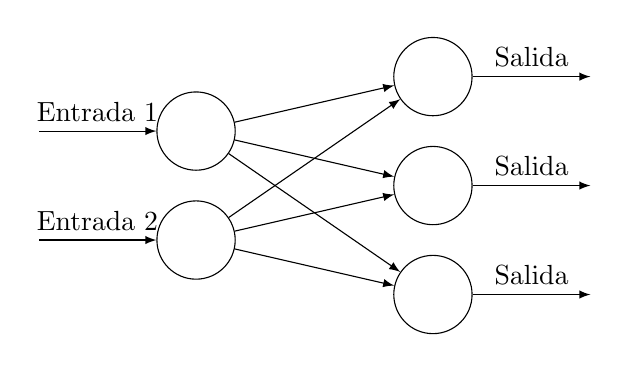
\begin{tikzpicture}[
plain/.style={
  draw=none,
  fill=none,
  },
net/.style={
  matrix of nodes,
  nodes={
    draw,
    circle,
    inner sep=10pt
    },
  nodes in empty cells,
  column sep=2cm,
  row sep=-9pt
  },
>=latex
]
\matrix[net] (mat)
{
|[plain]| &  \\
  & |[plain]| \\
 |[plain]| &  \\
& |[plain]| \\
|[plain]| &  \\
};
\foreach \ai [count=\mi ]in {2,4}
  \draw[<-] (mat-\ai-1) -- node[above] {Entrada \mi} +(-2cm,0);
\foreach \ai in {2,4}
{\foreach \aii in {1,3,5}
  \draw[->] (mat-\ai-1) -- (mat-\aii-2);
}

\foreach \ai in {1,3,5}
  \draw[->] (mat-\ai-2) -- node[above] {Salida} +(2cm,0);

\end{tikzpicture}


\end{document}